

% Configuración específica para anexos (continuando después de apéndices)
\renewcommand{\thechapter}{\Alph{chapter}}
\renewcommand{\chaptername}{Anexo}

% Aplicar estilo de página para anexos
\pagestyle{anexos}

%--------------------------------------------------------------------------------
\FloatBarrier
\chapter{Elementos en ArchiMate}\label{anexo:archimate-elementos}

% Introducción al anexo
Este anexo presenta una descripción detallada de los elementos y relaciones del lenguaje de modelado ArchiMate, proporcionando una referencia completa para la comprensión y aplicación de este estándar en arquitectura empresarial.

\noindent
Esta sección del anexo fue tomado del trabajo de grado de Michael Stiven Honores Quishpillo y Juan David Naranjo Sánchez titulado "Propuesta de Transformación Digital para la Gestión de la Información en el Proceso de Producción Establecido en la Organización Prefabricados JAMAR Validada a través de la Construcción de un Prototipo Funcional". 

\section{Elementos de negocio}

\begin{longtable}{|c|p{8cm}|}
\caption{Elementos de negocio en ArchiMate} \label{tab:elementos-negocio-archimate} \\
\hline
\textbf{Icono} & \textbf{Descripción} \\
\hline
\endfirsthead

\caption[]{Elementos de negocio en ArchiMate (continuación)} \\
\hline
\textbf{Icono} & \textbf{Descripción} \\
\hline
\endhead

\hline
\endfoot

\endlastfoot

\includegraphics{anexos/ARCHI/business/actor.png} & 
\textbf{Business Actor:} Una entidad que puede realizar un comportamiento dentro de la empresa, como una persona o una organización. \\
\hline
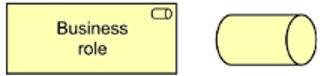
\includegraphics{anexos/ARCHI/business/rol.png} & 
\textbf{Business Role:} Define el conjunto de responsabilidades y comportamientos que un actor de negocio puede desempeñar. \\
\hline
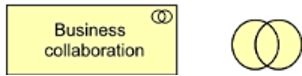
\includegraphics{anexos/ARCHI/business/colaboration.png} & 
\textbf{Business Collaboration:} Una agregación de dos o más roles de negocio que trabajan juntos para alcanzar un objetivo común. \\
\hline
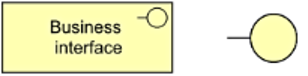
\includegraphics{anexos/ARCHI/business/interface.png} & 
\textbf{Business Interface:} Un punto de acceso donde un servicio de negocio es provisto a los actores de negocio. \\
\hline

\includegraphics{anexos/ARCHI/business/process.png} & 
\textbf{Business Process:} Un conjunto de actividades que logran un resultado específico para un cliente interno o externo. \\
\hline
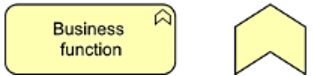
\includegraphics{anexos/ARCHI/business/function.png} & 
\textbf{Business Function:} Una agrupación de comportamientos con una base similar de recursos. \\
\hline

\includegraphics{anexos/ARCHI/business/interaction.png} & 
\textbf{Business Interaction:} Un comportamiento que describe la interacción entre dos o más roles de negocio. \\
\hline

\includegraphics{anexos/ARCHI/business/service.png} & 
\textbf{Business Service:} Un servicio que satisface una necesidad de un cliente, interno o externo, de la empresa. \\
\hline

\includegraphics{anexos/ARCHI/business/event.png} & 
\textbf{Business Event:} Algo que sucede y que afecta la continuidad de un proceso de negocio. \\
\hline
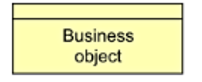
\includegraphics{anexos/ARCHI/business/object.png} & 
\textbf{Business Object:} Un concepto usado dentro de un dominio de negocio particular. \\
\hline
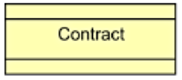
\includegraphics{anexos/ARCHI/business/contract.png} & 
\textbf{Contract:} Un acuerdo formal o informal que especifica los derechos y obligaciones asociados con un producto. \\
\hline
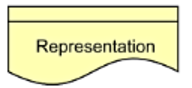
\includegraphics{anexos/ARCHI/business/representation.png} & 
\textbf{Representation:} Una forma perceptible de la información llevada por un objeto de negocio. \\
\hline
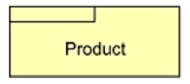
\includegraphics{anexos/ARCHI/business/product.png} & 
\textbf{Product:} Una colección coherente de servicios y/o objetos pasivos, acompañada de un contrato/conjunto de acuerdos. \\
\hline
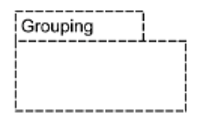
\includegraphics{anexos/ARCHI/business/grouping.png} &
\textbf{Grouping:} Un mecanismo para agrupar elementos relacionados en un modelo de arquitectura. \\
\end{longtable}

\section{Elementos de aplicación}

\begin{longtable}{|c|p{8cm}|}
\caption{Elementos de aplicación en ArchiMate} \label{tab:elementos-aplicacion-archimate} \\
\hline
\textbf{Icono} & \textbf{Descripción} \\
\hline
\endfirsthead

\caption[]{Elementos de aplicación en ArchiMate (continuación)} \\
\hline
\textbf{Icono} & \textbf{Descripción} \\
\hline
\endhead

\hline
\endfoot

\endlastfoot

\includegraphics{anexos/ARCHI/application/component.png} & 
\textbf{Application Component:} Una unidad modular que proporciona un conjunto de servicios relacionados en el contexto de aplicaciones. \\
\hline
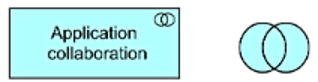
\includegraphics{anexos/ARCHI/application/collaboration.png} & 
\textbf{Application Collaboration:} Una interacción entre dos o más componentes de aplicación que trabajan juntos. \\
\hline

\includegraphics{anexos/ARCHI/application/interface.png} & 
\textbf{Application Interface:} Un punto de acceso a las funcionalidades de una aplicación. \\
\hline

\includegraphics{anexos/ARCHI/application/process.png} & 
\textbf{Application Process:} Un conjunto de comportamientos realizados por uno o más componentes de aplicación que alcanzan un objetivo específico. \\
\hline
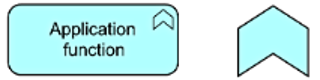
\includegraphics{anexos/ARCHI/application/function.png} & 
\textbf{Application Function:} Una agrupación de comportamientos relacionados en el contexto de aplicaciones. \\
\hline

\includegraphics{anexos/ARCHI/application/interaction.png} & 
\textbf{Application Interaction:} Un comportamiento que describe la interacción entre dos o más componentes de aplicación. \\
\hline

\includegraphics{anexos/ARCHI/application/service.png} & 
\textbf{Application Service:} Un servicio que una aplicación expone a su entorno. \\
\hline

\includegraphics{anexos/ARCHI/application/event.png} & 
\textbf{Application Event:} Algo que sucede y que afecta la continuidad de un proceso de aplicación. \\
\hline
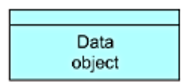
\includegraphics{anexos/ARCHI/application/object.png} & 
\textbf{Data Object:} Un objeto pasivo que es manipulado por un comportamiento dentro del contexto de aplicaciones. \\
\hline
\end{longtable}

\section{Elementos tecnológicos}

\begin{longtable}{|c|p{8cm}|}
\caption{Elementos tecnológicos en ArchiMate} \label{tab:elementos-tecnologicos-archimate} \\
\hline
\textbf{Icono} & \textbf{Descripción} \\
\hline
\endfirsthead

\caption[]{Elementos tecnológicos en ArchiMate (continuación)} \\
\hline
\textbf{Icono} & \textbf{Descripción} \\
\hline
\endhead

\hline
\endfoot

\endlastfoot
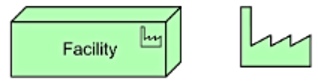
\includegraphics{anexos/ARCHI/technology/facility.png} & 
\textbf{Facility:} Un espacio físico o infraestructura utilizada para el alojamiento de recursos. \\
\hline

\includegraphics{anexos/ARCHI/technology/equipment.png} & 
\textbf{Equipment:} Un recurso físico que puede ser utilizado en los procesos de la empresa. \\
\hline

\includegraphics{anexos/ARCHI/technology/material.png} & 
\textbf{Material:} Recursos físicos o sustancias utilizadas o producidas por un proceso empresarial. \\
\hline
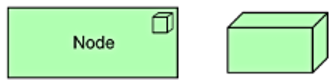
\includegraphics{anexos/ARCHI/technology/node.png} & 
\textbf{Node:} Un recurso computacional que aloja, manipula o interactúa con otros recursos y aplicaciones. \\
\hline

\includegraphics{anexos/ARCHI/technology/device.png} & 
\textbf{Device:} Un recurso físico que ejecuta software de sistema o componentes de aplicación. \\
\hline
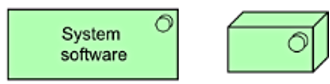
\includegraphics{anexos/ARCHI/technology/software.png} & 
\textbf{System Software:} Software que proporciona una plataforma para que las aplicaciones funcionen, como sistemas operativos y middleware. \\
\hline
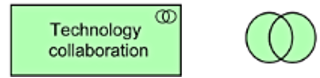
\includegraphics{anexos/ARCHI/technology/collaboration.png} & 
\textbf{Technology Collaboration:} Una interacción entre dos o más nodos o dispositivos que trabajan juntos. \\
\hline
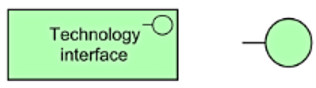
\includegraphics{anexos/ARCHI/technology/interface.png} & 
\textbf{Technology Interface:} Un punto de acceso donde un nodo o dispositivo ofrece su funcionalidad. \\
\hline
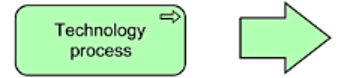
\includegraphics{anexos/ARCHI/technology/process.png} & 
\textbf{Technology Process:} Un conjunto de comportamientos tecnológicos que logran un objetivo específico. \\
\hline
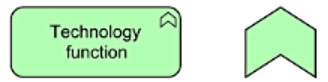
\includegraphics{anexos/ARCHI/technology/function.png} & 
\textbf{Technology Function:} Una agrupación de comportamientos tecnológicos relacionados. \\
\hline

\includegraphics{anexos/ARCHI/technology/interaction.png} & 
\textbf{Technology Interaction:} Un comportamiento que describe la interacción entre dos o más nodos o dispositivos. \\
\hline

\includegraphics{anexos/ARCHI/technology/service.png} & 
\textbf{Technology Service:} Un servicio ofrecido por la capa tecnológica a su entorno. \\
\hline

\includegraphics{anexos/ARCHI/technology/event.png} & 
\textbf{Technology Event:} Algo que sucede y que afecta la continuidad de un proceso tecnológico. \\
\hline

\includegraphics{anexos/ARCHI/technology/artifact.png} & 
\textbf{Artifact:} Un objeto físico de información utilizado o producido por un proceso de tecnología. \\
\hline
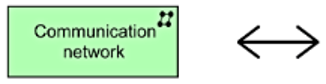
\includegraphics{anexos/ARCHI/technology/network.png} & 
\textbf{Communication Network:} Una infraestructura que permite la comunicación entre nodos y dispositivos. \\
\hline
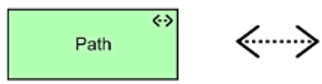
\includegraphics{anexos/ARCHI/technology/path.png} & 
\textbf{Path:} Una conexión que define el flujo de datos entre dos nodos o dispositivos. \\
\hline
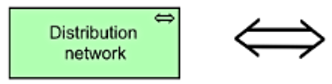
\includegraphics{anexos/ARCHI/technology/distribution.png} & 
\textbf{Distribution Network:} Una red que permite la distribución de productos o recursos a través de una infraestructura. \\
\hline
\end{longtable}

\section{Elementos de estrategia}

\begin{longtable}{|c|p{8cm}|}
\caption{Elementos de estrategia en ArchiMate} \label{tab:elementos-estrategia-archimate} \\
\hline
\textbf{Icono} & \textbf{Descripción} \\
\hline
\endfirsthead

\caption[]{Elementos de estrategia en ArchiMate (continuación)} \\
\hline
\textbf{Icono} & \textbf{Descripción} \\
\hline
\endhead

\hline
\endfoot

\endlastfoot

\includegraphics{anexos/ARCHI/strategy/meaning.png} & 
\textbf{Meaning:} Representa la importancia o propósito de algo dentro del contexto de la arquitectura empresarial. \\
\hline
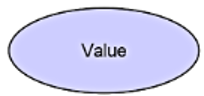
\includegraphics{anexos/ARCHI/strategy/value.png} & 
\textbf{Value:} Refleja el beneficio o utilidad percibida de un aspecto particular dentro de la organización. \\
\hline
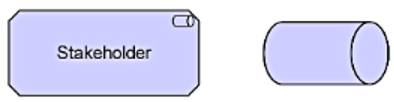
\includegraphics{anexos/ARCHI/strategy/stakeholder.png} & 
\textbf{Stakeholder:} Indica las partes interesadas o involucradas en la arquitectura empresarial, como individuos, grupos o entidades. \\
\hline
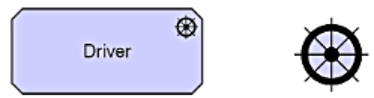
\includegraphics{anexos/ARCHI/strategy/driver.png} & 
\textbf{Driver:} Un factor que influye en el cambio dentro de la organización, motivando decisiones estratégicas o de implementación. \\
\hline
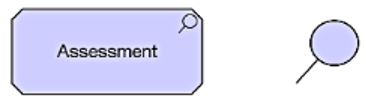
\includegraphics{anexos/ARCHI/strategy/assessment.png} & 
\textbf{Assessment:} La acción de evaluar o analizar la situación actual para identificar áreas de mejora u oportunidades. \\
\hline
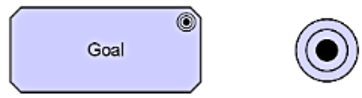
\includegraphics{anexos/ARCHI/strategy/goal.png} & 
\textbf{Goal:} Un resultado deseado que una organización intenta lograr para avanzar hacia su visión estratégica. \\
\hline
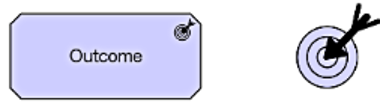
\includegraphics{anexos/ARCHI/strategy/outcome.png} & 
\textbf{Outcome:} El resultado tangible o intangible de una actividad, decisión o evento dentro de la organización. \\
\hline

\includegraphics{anexos/ARCHI/strategy/principle.png} & 
\textbf{Principle:} Una norma o regla fundamental que guía el comportamiento y las decisiones dentro de la organización. \\
\hline
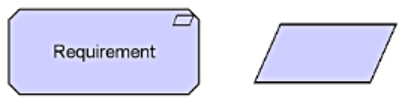
\includegraphics{anexos/ARCHI/strategy/requirement.png} & 
\textbf{Requirement:} Una condición o capacidad que debe cumplirse o poseerse por parte de un sistema, proceso o producto. \\
\hline
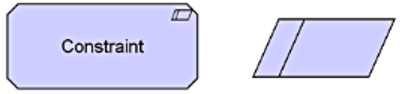
\includegraphics{anexos/ARCHI/strategy/constraint.png} & 
\textbf{Constraint:} Limitaciones o condiciones que restringen las opciones disponibles o el diseño de la arquitectura empresarial. \\
\hline
\includegraphics{anexos/ARCHI/strategy/resource.png} & 
\textbf{Resource:} Un activo o elemento disponible para su uso dentro de la organización, como personas, equipos o financiamiento. \\
\hline
\includegraphics{anexos/ARCHI/strategy/capability.png} & 
\textbf{Capability:} La habilidad o competencia que una organización posee para llevar a cabo actividades específicas de manera efectiva. \\
\hline
\includegraphics{anexos/ARCHI/strategy/stream.png} & 
\textbf{Value Stream:} La secuencia de actividades que entrega un producto o servicio de valor al cliente final. \\
\hline
\includegraphics{anexos/ARCHI/strategy/action.png} & 
\textbf{Course of Action:} Un plan o serie de pasos diseñados para alcanzar un objetivo específico dentro de la organización. \\
\hline
\includegraphics{anexos/ARCHI/strategy/work.png} & 
\textbf{Work Package:} Un conjunto de actividades o tareas agrupadas y asignadas a un responsable para su ejecución. \\
\hline
\includegraphics{anexos/ARCHI/strategy/event.png} & 
\textbf{Implementation Event:} Un evento o acción específica que marca el inicio o el fin de una fase de implementación dentro del proyecto. \\
\hline
\includegraphics{anexos/ARCHI/strategy/deliverable.png} & 
\textbf{Deliverable:} Un resultado tangible o intangible que se entrega al final de un proceso o fase de trabajo. \\
\hline
\includegraphics{anexos/ARCHI/strategy/plateau.png} & 
\textbf{Plateau:} Un estado o nivel estable alcanzado en la implementación de la arquitectura empresarial antes de avanzar hacia el siguiente nivel. \\
\hline
\includegraphics{anexos/ARCHI/strategy/gap.png} & 
\textbf{Gap:} La diferencia entre el estado actual y el estado deseado, que debe abordarse para alcanzar los objetivos estratégicos. \\
\hline
\end{longtable}

\section{Relaciones}

\begin{longtable}{|c|p{8cm}|}
\caption{Relaciones en ArchiMate} \label{tab:relaciones-archimate} \\
\hline
\textbf{Icono} & \textbf{Descripción} \\
\hline
\endfirsthead

\caption[]{Relaciones en ArchiMate (continuación)} \\
\hline
\textbf{Icono} & \textbf{Descripción} \\
\hline
\endhead

\hline
\endfoot

\endlastfoot
\includegraphics{anexos/ARCHI/relations/compostion.png} & 
\textbf{Composition:} Describe cómo los elementos se combinan para formar un elemento compuesto más grande en la arquitectura empresarial. \\
\hline
\includegraphics{anexos/ARCHI/relations/serving.png} & 
\textbf{Serving:} Indica cómo un servicio específico satisface las necesidades de uno o más componentes en la arquitectura empresarial. \\
\hline
\includegraphics{anexos/ARCHI/relations/triggering.png} & 
\textbf{Triggering:} Representa cómo un evento o condición inicia un proceso o comportamiento en la arquitectura empresarial. \\
\hline
\includegraphics{anexos/ARCHI/relations/and.png} & 
\textbf{(And) Junction:} Define cómo múltiples flujos deben cumplirse simultáneamente para continuar con un proceso o comportamiento en la arquitectura empresarial. \\
\hline
\includegraphics{anexos/ARCHI/relations/aggregation.png} & 
\textbf{Aggregation:} Muestra cómo varios elementos se agrupan en un conjunto mayor en la arquitectura empresarial. \\
\hline
\includegraphics{anexos/ARCHI/relations/flow.png} & 
\textbf{Flow:} Indica cómo los datos o el control se transfieren entre los elementos dentro de la arquitectura empresarial. \\
\hline
\includegraphics{anexos/ARCHI/relations/or.png} & 
\textbf{Or Junction:} Define cómo uno de varios flujos puede activar un proceso o comportamiento en la arquitectura empresarial. \\
\hline
\includegraphics{anexos/ARCHI/relations/assignment.png} & 
\textbf{Assignment:} Asigna responsabilidades, recursos o información a un elemento específico dentro de la arquitectura empresarial. \\
\hline
\includegraphics{anexos/ARCHI/relations/access.png} & 
\textbf{Access:} Describe cómo un elemento puede acceder o utilizar otro elemento dentro de la arquitectura empresarial. \\
\hline
\includegraphics{anexos/ARCHI/relations/influence.png} & 
\textbf{Influence:} Indica cómo un elemento afecta o modifica otro elemento dentro de la arquitectura empresarial. \\
\hline
\includegraphics{anexos/ARCHI/relations/realization.png} & 
\textbf{Realization:} Muestra cómo un elemento cumple con una especificación detallada o un requisito en la arquitectura empresarial. \\
\hline
\includegraphics{anexos/ARCHI/relations/association.png} & 
\textbf{Association:} Define una relación genérica entre dos elementos en la arquitectura empresarial. \\
\hline
\includegraphics{anexos/ARCHI/relations/specialization.png} & 
\textbf{Specialization:} Representa cómo un elemento se especializa o detalla más en un contexto particular dentro de la arquitectura empresarial. \\
\hline
\end{longtable}

%--------------------------------------------------------------------------------
\FloatBarrier
% Aquí se pueden agregar más anexos siguiendo el mismo patrón
% \chapter{Título del Anexo B}\label{anexo:nombre-anexo-b}
% \input{ruta/al/archivo.tex}


